\documentclass[11pt, letterpaper]{memoir}
\usepackage{HomeworkStyle}
\geometry{margin=0.75in}



\begin{document}

\begin{center}
	{\large Quiz 11.4 -- Electronic Spectroscopy}
\end{center}
{\large Name: \rule[-1mm]{4in}{.1pt}

\subsection*{Electronic Term Symbols}
Give the term symbol for the excited state of \ch{C2} with the following electronic configuration:

\noindent
$\sigma_g(1s)^2\sigma_u^\star(1s)^2\sigma_g(2s)^2\sigma_u^\star(2s)^2\pi_u(2p)^3\sigma_g(2p)^1$


\vspace{2em}\noindent
List all selection rules for electronic transitions

\vspace{3em}
\subsection*{Franck Condon Factors}
An electronic excitation significantly weakens and lengthens a chemical bond. Which vibrational state of the excited electronic state is likely to show the strongest transition? (Generally. I'm not looking for a particular value of $v^\prime$)

\vspace{3em}\noindent
The absorption and fluorescence spectra below show a few vibronic transitions. Give each peak a label indicating the initial and final vibrational states involved in each transition. Vibrational states of the ground electronic state should be referenced by their $v$ quantum number, and vibrational states of the excited electronic state should be referenced by their $v^\prime$ quantum number

\noindent
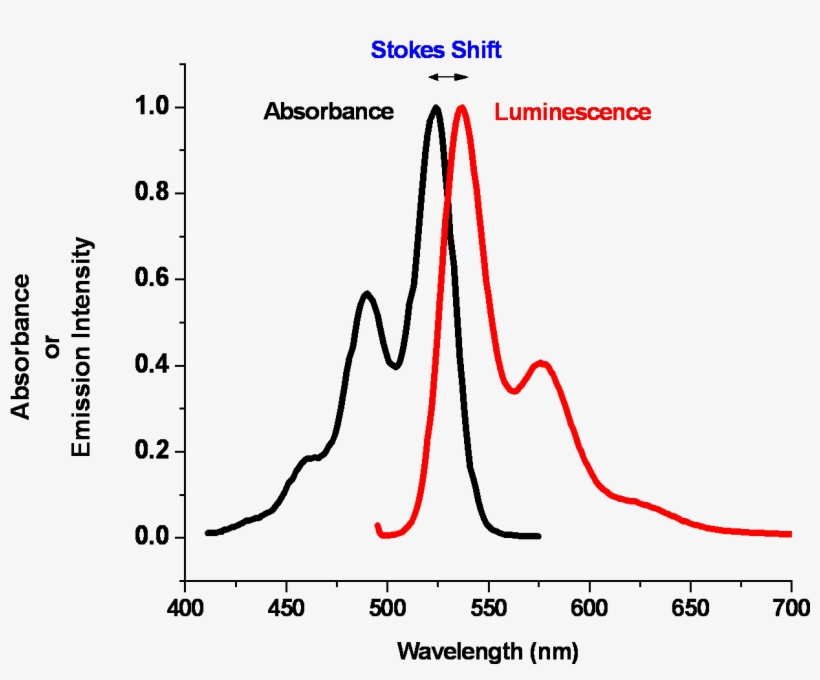
\includegraphics[width=0.5\linewidth]{Fluorescence}

\noindent
Next to the spectrum above, roughly sketch the potential wells and vibrational states for the electronic states involved.

\newpage
\subsection*{Decay Pathways}
Classify each decay pathway as \emph{internal conversion}, \emph{fluorescence}, \emph{phosphorescence}, or \emph{inter-system crossing}

\begin{itemize}
	\item $S_1 \rightarrow T_1$ (radiationless)

	      \vspace{1em}
	\item $S_1 \rightarrow S_0$ (radiative)

	      \vspace{1em}
	\item $S_1 \rightarrow S_0$ (radiationless)

	      \vspace{1em}
	\item $T_1 \rightarrow S_0$ (radiative)

	      \vspace{1em}
	\item $T_1,v^\prime=6 \rightarrow T_1,v^\prime=0$ (radiationless)
\end{itemize}

\newpage
\pagestyle{empty}
\addtocounter{page}{-1}
\section*{\emph{My Voice}}
\paragraph{By Rafael Campo}~
\begin{verse}
	To cure myself of wanting Cuban songs,\\
	I wrote a Cuban song about the need\\
	For people to suppress their fantasies,\\
	Especially unhealthy ones. The song\\
	Began by making reference to the sea,\\
	Because the sea is like a need so great\\
	And deep it never can be swallowed. Then\\
	The song explores some common myths\\
	About the Cuban people and their folklore:\\
	The story of a little Carib boy\\
	Mistakenly abandoned to the sea;\\
	The legend of a bird who wanted song\\
	So desperately he gave up flight; a queen\\
	Whose strength was greater than a rival king’s.\\
	The song goes on about morality,\\
	And then there is a line about the sea,\\
	How deep it is, how many creatures need\\
	Its nourishment, how beautiful it is\\
	To need. The song is ending now, because\\
	I cannot bear to hear it any longer.\\
	I call this song of needful love my voice.
\end{verse}
\end{document}
